\section{Machine Learning}\label{sec:machine_learning}
Machine learning is a part of the field of \ac{ai}. The focus is on extracting information from large amounts of data, with algorithms gradually improving themselves to mimic human learning~\cite{what-is-ml}.

The field of machine learning is itself divided into two main branches, Classical learning and Deep learning~\cite{ml-visual-explanation}.

% https://ischoolonline.berkeley.edu/blog/what-is-machine-learning/
% https://www.ibm.com/cloud/learn/machine-learning

\subsection{Deep Learning and Neural Networks} % TODO: need to proof read

Deep Learning includes various techniques that use neural networks. In the simplest form, neural networks consist of different so-called nodes, which are arranged as layers~\cite{neuralNet}.

The first layer, also known as the \enquote{input layer}, is the layer the input vector is applied to. If the input exceeds a certain value, the neuron is activated, i.e.\ it passes on an output.

In the next layers, which are called \enquote{hidden layers}, the outputs from all the nodes of the previous layer and a \enquote{bias layer} are computed in each node and the output is passed on. The bias layer consists of a single value that influences all nodes on a layer.

Finally, the last layer outputs the result of the computation. How strong each previous node influences the value of the current node is what the neural network is trained on.

Neural networks are particularly good at recognizing patterns in large unordered data, such as images, videos, and audio tracks. Examples of this include facial recognition or verifying hand signatures~\cite{neuralNet-applications}.

\newcommand{\neuralx}[2]{\(x_#2\)}
\newcommand{\neuraly}[2]{\(\hat{y}_#2\)}
\newcommand{\neuralh}[2]{\small \(h^{(#1)}_#2\)}
\begin{figure}[ht]
  \centering
  \caption[An example of a neural network]{A simple neural network with three input nodes and two output nodes.}
  \begin{neuralnetwork}[height=5]
    \inputlayer[count=3, bias=false, title=Input\\layer, text=\neuralx]
    \hiddenlayer[count=4, bias=true, title=Hidden\\layer 1, text=\neuralh] \linklayers{}
    \hiddenlayer[count=3, bias=false, title=Hidden\\layer 2, text=\neuralh] \linklayers{}
    \outputlayer[count=2, title=Output\\layer, text=\neuraly] \linklayers{}
  \end{neuralnetwork}\label{fig:neural_network}
\end{figure}

\subsection{Classical Learning} % TODO: writing
% https://towardsdatascience.com/deep-learning-vs-classical-machine-learning-9a42c6d48aa
Algorithms in the field of classical machine learning are largely based on statistical or probabilistic methods, which originated as pattern recognition in the 1960s. It has the advantage of being a fast method that does not require much computing power compared to deep learning algorithms~\cite{classical-ml}.

%! TODO: another paragraph

\subsection{Categories of Machine Learning}
There are different types of machine learning depending on the task and training data the machine learning model has to work with. % TODO: write better?
% Both deep learning and classical learning are dived into different categories which are based on the kind of task and training data the machine learning models have to work with.

Unsupervised learning is used on unlabeled data. Its main use is to organize the data or to make it more manageable. Tasks in this domain include clustering, which categorizes data based on similar data points, or association, which tries to find relationships between variables in a dataset~\cite{supervised-unsupervised-learning}.

Supervised learning on the other hand makes use of labeled data. This comes with the disadvantage that the structure of the data as well as the desired results have to be known~\cite{classical-ml}. Even though it increases the effort of the preparation of the training data, it also raises the accuracy of the model since it is trained to produce exactly the desired result.

% TODO: what and why labeled data?

% Reinforcement Learning  ~\cite{types-of-ml} %! TODO

\begin{figure}[ht]
  \caption[Different kinds of machine learning]{This picture shows the different types of machine learning and the way they are trained~\cite{types-of-ml}.} % TODO: is a more detailed description necessary?
  \centering
  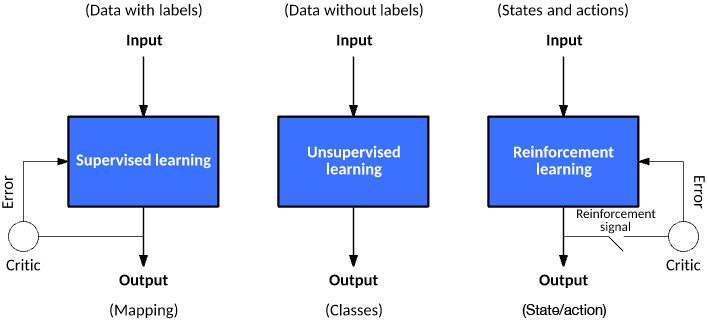
\includegraphics[width=\linewidth]{img/types_of_machine_learning.png}\label{fig:kinds_of_ml}
\end{figure}
